\RequirePackage[l2tabu,orthodox]{nag}

% TODO: decide if one-sided/two-sided
%\documentclass[headsepline,footsepline,footinclude=false,fontsize=11pt,paper=a4,listof=totoc,bibliography=totoc,BCOR=12mm,DIV=12]{scrbook} % two-sided
\documentclass[headsepline,footsepline,footinclude=false,oneside,fontsize=11pt,paper=a4,listof=totoc,bibliography=totoc]{scrbook} % one-sided

\PassOptionsToPackage{table,svgnames,dvipsnames}{xcolor}

\usepackage[utf8]{inputenc}
\usepackage[T1]{fontenc}
\usepackage[sc]{mathpazo}
\usepackage[american]{babel}
\usepackage[autostyle]{csquotes}
\usepackage[%
  backend=bibtex,
  url=false,
  style=numeric,
  maxnames=4,
  minnames=3,
  maxbibnames=99,
  firstinits,
  uniquename=init]{biblatex} % TODO: adapt bibliography style
\usepackage{graphicx}
\usepackage{scrhack} % necessary for listings package
\usepackage{listings}
\usepackage{lstautogobble}
\usepackage{tikz}
\usepackage{pgfplots}
\usepackage{pgfplotstable}
\usepackage{booktabs}
\usepackage[final]{microtype}
\usepackage{caption}
\usepackage[hidelinks]{hyperref} % hidelinks removes colored boxes around references and links
\usepackage[toc,nonumberlist,acronym]{glossaries} % TODO: remove if glossary not needed
\usepackage{subcaption}
\usepackage{algorithm,algpseudocode}
\bibliography{bibliography/literature}

\setkomafont{disposition}{\normalfont\bfseries} % use serif font for headings
\linespread{1.05} % adjust line spread for mathpazo font

% Settings for glossaries TODO: remove the following block if glossary not needed
\renewcommand{\glsnamefont}[1]{\normalfont\bfseries #1} % use serif font for glossary entry titles
\makeglossaries{}

% Settings for pgfplots
\pgfplotsset{compat=1.9} % TODO: adjust to your installed version
\pgfplotsset{
  % For available color names, see http://www.latextemplates.com/svgnames-colors
  cycle list={CornflowerBlue\\Dandelion\\ForestGreen\\BrickRed\\},
}

% Settings for lstlistings
\lstset{%
  basicstyle=\ttfamily,
  columns=fullflexible,
  autogobble,
  keywordstyle=\bfseries\color{MediumBlue},
  stringstyle=\color{DarkGreen}
}

% Basic information for cover & title page
\newcommand*{\getUniversity}{Technische Universität München}
\newcommand*{\getFaculty}{Fakultät für Informatik}
\newcommand*{\getTitle}{Implementation and Evaluation of a Persuasive Mobile Food Recommendation System}
\newcommand*{\getTitleGer}{Implementierung und Evaluierung eines persuasiven mobilen Ernährungs-Empfehlungssystems}
\newcommand*{\getAuthor}{Muhammad Kabir Khan}
\newcommand*{\getDoctype}{Master's Thesis in Informatics}
\newcommand*{\getSupervisor}{Prof. Johann Schlichter, Ph.D.}
\newcommand*{\getAdvisor}{M.Sc. B\"eatrice Lamche}
\newcommand*{\getSubmissionDate}{June 30, 2015}
\newcommand*{\getSubmissionLocation}{Munich}

% TODO: add custom commands etc.

% TODO: remove if glossary not needed
\newglossaryentry{computer}
{
  name=computer,
  description={is a machine that\ldots}
}

\newacronym{tum}{TUM}{Technische Universität München}


\begin{document}

\begin{titlepage}
  % HACK for two-sided documents: ignore binding correction for cover page.
  % Adapted from Markus Kohm's KOMA-Script titlepage=firstiscover handling.
  % See http://mirrors.ctan.org/macros/latex/contrib/koma-script/scrkernel-title.dtx,
  % \maketitle macro.
  \oddsidemargin=\evensidemargin\relax
  \textwidth=\dimexpr\paperwidth-2\evensidemargin-2in\relax
  \hsize=\textwidth\relax

  \centering

  \vspace{40mm}
  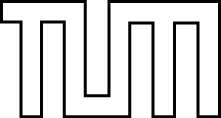
\includegraphics[width=40mm]{logos/tum}

  \vspace{5mm}
  {\huge\MakeUppercase{\getFaculty{}}}\\

  \vspace{5mm}
  {\large\MakeUppercase{\getUniversity{}}}\\

  \vspace{20mm}
  {\Large \getDoctype{}}

  \vspace{15mm}
  {\huge\bfseries \getTitle{}}

  \vspace{15mm}
  {\LARGE \getAuthor{}}

  \vspace{20mm}
  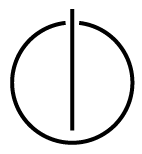
\includegraphics[width=20mm]{logos/faculty}
\end{titlepage}


\frontmatter{}

\begin{titlepage}
  \centering

  \vspace{40mm}
  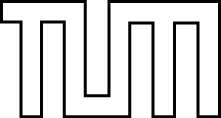
\includegraphics[width=40mm]{logos/tum}

  \vspace{5mm}
  {\huge\MakeUppercase{\getFaculty{}}}\\

  \vspace{5mm}
  {\large\MakeUppercase{\getUniversity{}}}\\

  \vspace{20mm}
  {\Large \getDoctype{}}

  \vspace{15mm}
  {\huge\bfseries \getTitle{}}

  \vspace{10mm}
  {\huge\bfseries \getTitleGer{}}

  \vspace{15mm}
  \begin{tabular}{l l}
    Author: & \getAuthor{} \\
    Supervisor: & \getSupervisor{} \\
    Advisor: & \getAdvisor{} \\
    Submission Date: & \getSubmissionDate{} \\
  \end{tabular}

  \vspace{20mm}
 % 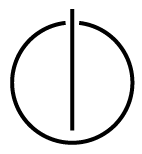
\includegraphics[width=20mm]{logos/faculty}
\end{titlepage}

\thispagestyle{empty}
\vspace*{0.8\textheight}
\noindent
I assure the single handed composition of this \MakeLowercase{\getDoctype{}} only supported by declared resources.

\vspace{15mm}
\noindent
\getSubmissionLocation{}, \getSubmissionDate{} \hspace{5cm} \getAuthor{}

\cleardoublepage{}

\addcontentsline{toc}{chapter}{Acknowledgments}
\thispagestyle{empty}

\vspace*{2cm}

\begin{center}
{\usekomafont{section} Acknowledgments}
\end{center}

\vspace{1cm}

%TODO: Acknowledgments
I would like to thank to my advisor Beatrice Lamche, who always give me her valuable advice and her guide during the phase of my research. I am also very grateful to Geogh Gorh and Silvia Kolssa for there advises in continuing my research.\newline

I also recognize all the participants how took part in user study to evaluate my work. I am also thankful to my dearest friend Muhammad Mudassir Khan for his valuable advices. Least but not the least my family, because of their prayer I would able to make it.

\cleardoublepage{}

\chapter{\abstractname}

%TODO: Abstract



\microtypesetup{protrusion=false}
\tableofcontents{}
\microtypesetup{protrusion=true}

\mainmatter{}

\chapter{Introduction}
\pagenumbering{arabic}%Ab hier, werden arabische Zahlen benutzt
\setcounter{page}{1}%Mit Abschnitt 1 beginnt die Seitennummerierung neu.
\thispagestyle{empty}

The motivation behind this Master Thesis is to implement and evaluate a Healthy Food Recommendation System for Mobile. In the beginning, it provides overview and give the reasoning about the selection of system. Relevant background and related work is presented, Followed by the development and design process together with the evaluation process will be presented. \newline
This chapter will enlighten the motivation behind developed system in Section 1.1. Followed by goals in Section 1.2. Whereas Section 1.3 will provide a brief outline on structure of thesis.

\section{Motivation}\label{motivation}

Rapid innovation and significant advancement in the field of technology and scientific research has made smartphone a primary computing and communication device. Smartphone is now become a necessity of life and people use it as an assistant for their day to day work. According to latest survey more than half of Internet traffic is accounted by mobile device. Enhancement in communication technology and flexible data option provided by network operators has increase relevance of interactive mobile applications. Packed with hundreds of features smartphone use different applications for variety of functionalities which required internet connectivity. Furthermore, smartphone support touch screen and rich support of multimedia and other application take the user experience to the next level.\newline

Suggestions are the important factor of our day-to-day life. From watching a movie, to cooking and to on shopping. We need valuable advice. Recommendations are always helpful in choosing a better alternative. It not only save time but also minimize the individual's effort.\newline

Recommender system are increasingly popular now are days. Form e-comers to movie websites, they not only help to increase business but also behave an personalize user preference assistance. Another aspect of describing Recommend system is filtering technology that user to filter suggests the information to user according to his taste. In order words we can also say that Recommender systems are the smart search engine, which suggest result by, compare different items with each other. Research and advancement are going on this domain in order to improve the quality of recommendations. \newline 
The most important goal for recommendation system designers is user willingness to peruse recommendation provided by the system. Fundamental process of recommendation is finding and conceptualizing relationship of item, current context and how the message is communicated, opens up the way of persuasiveness in recommendations.\newline

Services provided by recommendation system through e-commerce to cooking are numerous in nature. Searching of products returns an overwhelming set of options. For instance, Comparing and Filtering of products among irrelevant set and find the suitable product. Such techniques work fine with web interface, whereas, smartphones they are not very useful due to hardware limitations. Critique-based recommendation helps in revision and acquisition of user preference, in order to improve quality of recommendations.\newline
One the basic need is Food among human. Good health represents proper dietary habit. However, diet plan is always based on person’s physical conditions like gender, weight, age and health status. Furthermore, taste and food preference is differ among individuals. Therefore, creating balance dietary plan based on individuals taste and health preference is always challenging.\newline
The World Health Organization [1] is predicting that the number of obese adults worldwide will reach 2.3 billion by 2015 and the issue is attracting increased attention. Therefore, electronic food management systems have become a hot topic and, are under consideration to replace traditional paper based program. Idea of using electronic devices for health related matter is not new; similar devices are in use by patients for medical reasons e.g. Glucometer, and blood pressure monitor. People want, to carry better life style and to live healthy. Therefore popularity of food monitoring systems is getting popular.  These systems are not only providing valuable services but hold user preferences and keeps history to provide more personalize recommendations. Recommendations are based on food ratings and browsing histories.\newline

Food recommendations have gotten a tremendous amount of success and still in research phase for further improvement. Along with significant advancement and feature set like similar recipes, recipe nutrition detail, where to buy ingredients from some research, some wholes are still remaining. Indeed recommendation techniques like collaborative, content and knowledge based filtering are good for job done. But food domain is not quite simple. User preference and taste not only change by their mood but much more depend upon their health. Therefore, Active learning and critiquing techniques are required to improve better recommendation. So that user can give their feed back and get what ever his preferences are. Mostly approaches are done critiquing by using rating of recipes and generate their result by using celebrative or content based filtering. Similarly, knowledge based filter digs some more; here rating is based on ingredients. Furthermore, persuasion of recommendation is always not guarantied in all cases. Clearly the system is not able to provide the best recommendations due to its detachment from the current situation; what is lacking in these approaches are intersection of persuasiveness, active learning and critiquing and last but not the least user preference context.\newline

This work focuses on generation of health food recommendation on a mobile platform. Recommendation relies on user context, which allow user to critique, based on ingredients and recipes depends on his health and taste through which system will perform active learning. Lastly all recommendations should be persuasive in nature. in order to achieve persuasiveness in recommendations, we focus on user interface and the explanation of recommendation. Which helps user to get an idea why system generates this recommendation to me.\newline

The following short description of the target scenario will illustrate the driving idea behind this research project.\newline

 \textit{John is a software engineer and very health conscious. He has a tight schedule due to work and gym but loves to cook. He wants to keep track of his diet depends on his taste and preferences. Furthermore, he wants try out some new food base on his time schedule}\newline

\section{Goals}

On the basis of scenario, describes in last section, this work reflects the goals which are stated below:\newline
A recommendation is valuable if it interests the user. To determine the generated recommendation is according to user interest entails to our first primary goal, which is offering Persuasive recommendations. Major factors should be considered before given suggestion is Message and Source. Therefore our Second goal is to implement Active Learning and Critiquing approach to justify our suggestion. Since Critiquing relies on context that’s why it is important to understand the Consumption and Accessibility context which infers our third goals.  Similarly understanding the food ontology refers in scenario helps us to understand forth goal of system. Finally how the user will interact with his device conveys our last goals, which is Mobile user interface.\newline

To achieve primary goals there are several other interesting secondary goals, which facilitate, how our primary goals should be achieved. Starting with the research phase, which includes question and answers to user how they want to use such system in order to achieve better usability. Next focus on existing search work how the other system implements food recommendation scenarios, finding out what are their weakness and strengths. Food ontologies understanding how they are interrelate with other. What factor in which recipes are dependent on in order to develop strong system. Understanding user context which time he prefers which recipe. Furthermore, it is important to research on what researches and related work are out there under Persuasive and Active learning and Critiquing system to grab the understanding, how we can get inspiration from their valuable approaches and work. Finally focus on user experience of such application is one of challenging task, how and where to show the important aspects of recipe in our interface, so that it is easy to learn and has improved usability in comparison with current market applications.\newline
Once the research phase has done next step to collect the functional and non-functional requirement of the system, which is collected by interviewing friends and family voluntaries. Once the system is build it has been tested with gathered functional and non-functional requirement and find out the limitation or boundary conditions of system. More over iOS client needs to be test with given requirement additionally user satisfaction should be required for usability test.\newline

Finally, evaluation of developed prototype by user study. In order to clarified the methodologies and processes followed by our selected approaches. After finishing the evaluation reflected results leads to potential improvements and opens up the new direction of research.\newline

\section{Outline}

Division of this thesis is split up into six chapters. \textit{Chapter1} contains introduced the ideas, motivations and goals.\newline

\textit{Chapter2} starts with background in which some definitions and classification of recommendation systems, Followed by different types of profiling and contexts that impact on recommendations. Furthermore, in related work section, pervious work of Persuasiveness, Critiquing and Personalized food recommendation techniques have been discussed.\newline

\textit{Chapter3} explains the Profiling and Context in details along with factors of recommendations. Moreover it covers algorithms that are used to develop the system.\newline

\textit{Chapter4} discuss the System design and architecture phase, which hold the all ERD, components view, servers on which system depend. In the end of the chapter API calls are mentioned which are provided by server.\newline

\textit{Chapter5} elaborates how the user study has been conducted by mentioning the goals, methods, and testing framework along with the dataset. In the end of this chapter measured results and discussion is mention.\newline
  
\textit{Chapter6} will summarizes the achievements and gives clues about further development and research.\newline


\chapter{Background and Related Work}

This chapter will establish the foundation of Persuasive recommendation system along with active learning and critiquing approach. Prior to in depth analysis, it will provide important background information along with some required definitions. Additionally, related work will presented, as the chapter proceed further to the end..\newline

\section{Definitions}

\subsection{Recommender System}

Recommender Systems (RS) are search tools, which supports user decision-making by providing the suggestion that, are according to their interests. Such systems are widely uses from social networking through e-commerce sites in order to achieve different purposed. In e-commerce site, they help not only to serve the customer by suggesting items according to their preferences but also support business to improve in its sale. On the other hand in social network site, to suggest friends or pages like according to user preferences. According to Ricci [Ricci, 2010] "RS are information search tools that have been recently proposed to cope with the "information overload" problem, i.e., the typical state of a web user, of having too much information to make a decision". Proposed solution [Resnick and Varian, 1997] is an intelligent system that suggests the product or service that fulfill the user’s preference in given context or situation. Suggestions provided by such systems are depended on the model how they are keeping information. Majority of RS are typically community based. In this kind of modeling suggestions are depend about item popularity among the user. Where popularity is calculated by ratings. Important question that arise in such systems are to find item accuracy according user preferences. On the other hand Personalized models are used that depends on the various factors which includes user’s preferences, history of bought/liked items, or the items the user has ranked in the past. Various techniques are use in the developing of recommender system. Classification of recommendation systems [Ricci, 2001] will be discussed as follows.

\subsubsection{Content-based filtering}

In this technique recommendations are based on user preference. System recommend items that similar to one is liked by user. Item similarity is calculated by features associated with the compared items [Ricci , 2001]. For example, if a user has rated positively recipe A under the category of sweet then next suggestion that is provided by the system is one which is similar to one user has like before.

\subsubsection{Collaborative-based}

Collaborative filtering is technique in which system find the correlation between item and user based opinions of other users which having a similar taste in past [Shapira , 2001]. Initially system calculates all similar taste users for the current user and calculate the recommended item that contains either rated or liked by other users having similar taste. Importantly in this approach item speciation will not be considered. For instance, if user like recipe A then next recommendation would be recipe that there are other users who liked recipe A also liked recipe B.

\subsubsection{Demographic}

Recommendations are generated according to user demographic profile. Recommendations can be produced for different demographic niches by combining the ratings of users in demographic clusters [Mahmood, 2007]. For example, suggestion provided by the systems are shown according to user’s age. 

\subsubsection{Knowledge-based}

In knowledge-based systems item recommendation is based on domain specific knowledge, which justifies how certain item features meet according to user’s preferences [Ricci , 2001]. Importantly, it uses predication techniques namely Case-based reasoning which reuses the cases past cases that are similar to current case in order to identify item set of recommendation.

\subsubsection{Community-based}

Type of recommendations provided by this kind of system based on preference of user friends. According to Ricci research [Ricci, 2001], People tend to rely more on recommendations provided by friends rather than on recommendations from anonymous individual having similar taste. Such type of RS model relies on user’s social relations including preference of user’s friends. Suggestions depend on rating that is provided by user’s friends.

\subsubsection{Hybrid Recommender Systems}

Hybrid system is a fusion of any two or more techniques motioned above. Ricci [Ricci , 2001] explains the motivation behind such system to avoid the limitation of one technique. For instance, Collaborative filtering have cold startup problem i.e. they are unable to suggest those items, which have no ratings. On the other hand Content-based doesn’t have such limitation by combination of both approach new hybrid system can be formed. Similarly, Burke [Burke, 2007] proposed the combination techniques to create a new hybrid system.

\subsubsection{Traditional Recommender Systems Limitations}

Traditional recommendation approaches focus on the recommending the most relevant item according to user preferences without considering any context information for example place and time. Problem occurs when user interest with the system with a particular context and preference may be change for another context[Adomavicius 
, 2012]. For instance, User wants to cook dinner for his guests expects different recommendations as compared to searching for himself/herself.

\subsection{Contexts}

\subsection{User Profiling}

\subsection{Food Profiling}

\subsection{Conversation Critiquing and Active Learning}

\subsection{Persuasive Recommedations}

\section{Related Work}

\subsection{User's Food Preference Extraction for Personalised Cooking Recipe Recommendation}

\subsection{Knowledge Base Framework for Development of Personalised Food Recommendation System}

\subsection{Interactive Explanations in Mobile Shopping Recommender Systems}

\subsection{Active Learning Strategies for Exploratory Mobile Recommender Systems Interactive Explanations in Mobile Shopping Recommender Systems}

\chapter{Design Decisions}

This chapter will provide the explanation about the design decisions that we have made to develped our system. It will also highlight how they intereact with each other in order to achieve the goals of this thesis. The chapter begins with explanation of profiling approaches, followed by impacts of context, critiquing and persuasion.

\section{User Profile}

One the core component of a system is to recommend user food that suits to his preferences, which can be gathered by profiling a user. In our system we followed a hybrid approach to build a user profile. Demographic information of a user is implicitly fetched from his Facebook account. The reason behind following implicit profiling approaches is to get user information without bothering them. This allows system to have up to date information about them.  However, it has been noticed that people are reluctant to those systems that request permission to access their social network activity information. Knowing these concerns, we only ask users to permit access to their basic information. Following are the acquired attributes from Facebook profile.

\begin{enumerate}
	\item Birthday
	\item Email	
	\item FirstName
	\item LastName
	\item Gender
	\item Name
	\item Profile Link
	\item UserId
\end{enumerate}

Moreover, explicit profiling techniques are used to gather users' contextual information and their preferences. While explicit profiling reveals accurate information, there however exist shortcomings in this technique. It demands user’s time and willingness to provide the data by filling the long forms, which seems to be tedious to the users. As the system is Knowledge based Personalized recommender, this problem has to be dealt efficiently because the recommendations produced by the system are highly influenced by user feedback. Therefore instead of making a user to provide all the information, we collect this data by using interactive forms based, which includes simple toggling, rating and selection mechanism that also increase the usability of the system.

\section{Food Profile}

Food recommendation is the basic research area of this thesis. Based on this approach our research is to provide recommendation according to both individual‘s dietary needs and preferences. Understanding food domain is very complex and challenging task when its come to recommender domain. User’s selection of a recipe is highly depends on it’s ingredients. Also there are some other factors which includes cooking methods, ingredient costs and availability, complexity of cooking, preparation time, nutritional breakdown, ingredient combination effects, as well as cultural and social factors \cite{freyne2010recommending}. Our research starts with in finding out how popular websites are dealing in this domain and structuring the recipes. So that we can get inspiration about the important features that user are looking for while he interacts with such system. Next chore of our research is to build a recipe database therefore we need a provider-API that ensures a large number of recipes. Among these APIs two notables with impressive meta-data about recipes are:

\begin{enumerate}
	\item Yummly API.
	\item BigOven API.	
\end{enumerate}

Both services are crowd-source driven, highly recommended in food domain and are offering almost the same data set. Next step to find the best suited API for our research therefore we preformed some experiments targeted to comparison between both selected API. Result of this experiment showed that Yummly API is not providing cooking description. On the other hand BigOven API doesn’t support recipe’s nutritional information and have limited number of calls per hour for student account. Regarding selection of API our focus was, it should provide all the relevant information about the recipes required by our research, in order to avoid any dependency. Considering mentioned fact we decided to choose BigOven API.\newline

Concerning about the attributes of food profile we followed the common approach that recipe have some important key attributes like cooking methods, ingredient preparation time, nutritional breakdown \cite{freyne2010recommending}.  However we are unable to get nutritional information due to API’s constrain, as discussed early, but in our data model we are considering it for future research purpose.  Figure \ref{fig:ch2_food_profile} illustrates the key attributes of food profile which is a common fashion for representing a recipe. We followed an hybrid approach \cite{suksom2010knowledge}
\cite{teng2012recipe} \cite{freyne2010recommending} for our personalize knowledge bases food recommendation system. Recipe’s ingredients are the primary factor on which recommendations are relied. 

\begin{figure}[h]
	\centering
	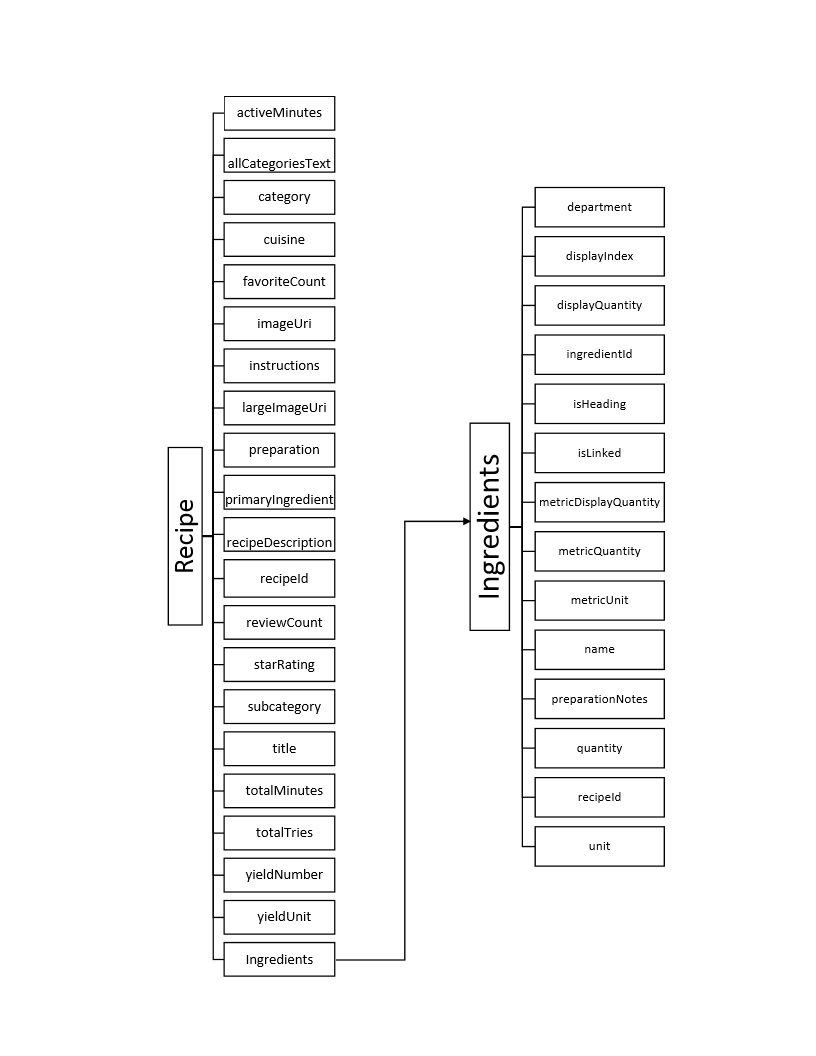
\includegraphics[width=.7\linewidth]{figures/ch2_food_profile.png}
	\caption{Attributes in Food Profile} 
	\label{fig:ch2_food_profile}
\end{figure}

\subsubsection{Assumption}

In order to simplify evaluation of recipe recommendation, System assumed that liking and disliking of ingredients by user is based on his dietary needs and health preferences. Suppose user does not like a particular ingredient let’s say “X”, therefore system learns from user’s critique and eventually avoids such recipes, which have "X" as an ingredient in it.

\subsubsection{BigOven API}

BigOven API provides all the information about the recipe in a well-structured and well documented manner. Along with the high number of recipes, they offer functionalities including  \textit{Search, Display Recipes, Recipe review, Grocery List and Rest-based API support}. For this thesis we focus only few of them to develop a database of your system.  Following are some API calls that are implemented in our system.


\begin{enumerate}
	\item \textbf{Reading a Recipe.}\newline \newline
	The Recipe object refers to a recipe within the BigOven collection.\newline \newline
%%%%%%% Request
	\textbf{URL request:}\newline 
	\textit{GET http://api.bigoven.com/recipe/{id}?api\_key="bigOvenApiKey"}
	\newline 
%%%%%%% Table	
	\begin{table}[ht]
		\centering % used for centering table
		\begin{tabular}{p{3cm} p{6cm} p{3cm}}  % centered columns (3 columns)
			\hline\hline %inserts double horizontal lines
			Parameter & Description & Required \\ % inserts table
			%heading
			\hline % inserts single horizontal line
			id & Primary key(ID) of recipe & Yes \\ 
			api\_key & Your api key issued to you by BigOven & Yes \\ 
			\hline %inserts single line
		\end{tabular}
		\caption{Bigoven- Reading a Recipe.}
		\label{table:bigoven-reading-recipe}
	\end{table}
%%%%%%% End Table		
	
	\item \textbf{Recipe Search Results.}\newline \newline
	The Recipe Search Result object is a collection of results for a given recipe search query.\newline \newline
	%%%%%%% Request
	\textbf{URL request:}\newline
	\textit{GET http://api.bigoven.com/recipes?title\_kw=" keyword"\&pg="page"\&rpp="resultPerPage"\\
	\&api\_key="bigOvenApiKey"	} \newline 
	
	%%%%%%% Table	
	\begin{table}[ht]
		\centering % used for centering table
		\begin{tabular}{p{3cm} p{6cm} p{3cm}}  % centered columns (3 columns)
			\hline\hline %inserts double horizontal lines
			Parameter & Description & Required \\ % inserts table
			%heading
			\hline % inserts single horizontal line
			title\_kw & Title keyword being searched for & No \\ 
			pg & Cureent Page to be fetched & No \\ 
			rpp & Number of results in page & No \\ 
			api\_key & Your api key issued to you by BigOven & Yes \\ 
			\hline %inserts single line
		\end{tabular}
		\caption{Bigoven-  Recipe Search Results}
		\label{table:bigoven-recipe-search-results}
	\end{table}
	%%%%%%% End Table	

\end{enumerate}

\section{Contexts}

Any information that can be used to characterized the situation of entity known as Context. For instance person, place\cite{ abowd1999towards}.  Incorporation of context in recommendation system leads to improve the quality of recommendation. System that uses context to provide relevant information is called context-awear system.  Lee, H. et al., \cite{lee2005context} classified context based on existing classification and definition in mobile domain. He categorized contextual information into five categories and further divided in to sub categories Figure\ref{fig:ch2_lee2005context} is a illustration of his classification.\newline 

\begin{figure}[h]
	\centering
	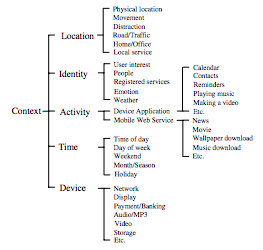
\includegraphics[width=.55\linewidth]{figures/ch2_lee2005context.png}
	\caption{Context hierarchy of the Mobile Web.} 
	\cite{lee2005context}
	\label{fig:ch2_lee2005context}
\end{figure}

\textit{Location} not only refers to user’s current location but also what objects are nearby to user such as destination, restaurants and local services. Also it tells about the state of the user like he is moving to staying with respect to specific place, such as home or office. \textit{Identity} is the representation of person’s interests e.g. emotional state, preferred keyword , usage history and social network. \textit{Activity} describe current usage of a mobile device,  for instance which services are using by user. \textit {Time} refers to  the current time as per system clock e.g. time of device, also time elaborates in terms of day, week, month of the year. \textit{Device} is a combination of hardware, software and network features that are provided by mobile for example Operating system version, Camera and Color.  Network explains as cellular technology and wireless interface such as 3G, LTE and Bluetooth.\newline
	
Considering Lee, H. et al.,’s classification \cite{lee2005context} as a foundation, different attributes of  context used in our system are discussed in the following forthcoming section.

\subsection{User Context}

As discussed in earlier section, user context create huge impact while recommendations are made.  Briefly, user context refers to the current activities of user. for example, what is the user during a specific circumstances. \textit{Cuisine’s Recipe and User Health and taste} are considered as  user interest in our system. User need to define \textit{ Cuisine’s Recipe} while he wants to interact with the system in order to narrow down the recommendation  according to selected food type. Since all the recipes are categorize as, drinks, breakfasts and appetizer.  Also \textit{User Health and taste}  context is gathered by user feedback. Considering user health and taste preferences system will not add those recipes, which do not matches to his profile. 
	
\subsubsection{User's Health Context}

Elaborating more about user’s health. Definition of health is totally depending on in which perspective it is evaluating. Initially we want to calculate health by the help of nutrition information provided by the recipe but due to API constrains we are unable to define in this manner. However we come with another approach, which sound more intuitive and simple to measure health i.e. BMI (Body Mass Index). BMI depends on Person’s age, height and weight. It is use to measure body fatness and health of individual. By the BMI we can record how much calories he eat and how much he required maintaining his BMI. We mocked the information of calories and exercise information in our explanation to measure the effect of persuasion. 


\subsection{Accessibility Context}
	
Accessibility context is a combination of “Activity” and “Time” according to above mentioned classification \cite{lee2005context}.  Following are the attributes which are related to our system: \textit{Cooking Time} indicates that how much time user have for cooking, so that system can recommend him only those recipes which are related to user’s preferred cooking time. \textit{Recipe’s Next Cooking Time} assume the recipe that user most likely to cook. System will not recommend the particular recipe which is already cooked by the user during a week. Assumption behind one-week cooking gap for a cooked recipe was to provide verity of recipes to user to maintain his interest. 
	

\subsection{Device Context}
	
Focus of this research is requires a mobile platform. Android, iOS and Windows phones are the three considered option. We selected iOS platform and chose iPhone as a selected device for developing our prototype. The reason behind the selection of iOS, was to develop a high fidelity UI which is intuitive and useable, by considering all the User interface guide lines provided by Apple Inc. iOS version that is required by our app is minimum 8.3. However, client side code written in swift programming language, highly recommended by Apple Inc.


\section{Critiquing}

Elicitation of user preference is the key step of recommendation system. There are many simple approaches for accusation of user preferences and transform it into user model. Traditionally, these were acquired explicitly where user need to fill a form and mentioned his wants and need. However, it has been noticed users avoid in filling information about themselves. Using these approaches result less knowledge about user preference and poor recommendations. To solve these problems two methodologies have been suggested. In first approach accusation of user’s preferences takes place by analyzing of user’s navigation behavior. This assumption that user always visit his interested item. Advantage is requiring lower user effort. While shortcomings are: (1) It depends understating of domain specific knowledge because user actions are translated into user preferences model. (2) Noise existence because preference and context of a person may differs from another person.\newline

Second is conversational approach a new paradigm for the collection of user preference and redefines human-computer interaction. Such systems are based on interaction cycles in order to gather preferences about the users. At interaction cycle, the system can either ask the user a preference or propose a product to the user. The user can reply either by answering to the question posed or by criticizing the system proposal.\cite{ricci2005critique}\newline

Moreover, Critiquing by conversational approach is not enough in our case. It can answer to the cold startup problem and are unable to deliver quick results. Therefore Active Learning (AL) is the additional approach, which is used by our system in order to quickly deliver good results without preexisting knowledge about user preferences. \cite{lamche2014active}. We followed Model-based AL methodology in order to construct user model regarding ingredient and recipe selection, avoid expected error in model. As far as AL mode is concerned we followed the Sequential model states as: recalculate the rating of item once user rated that specific item. In our case ingredients and recipe \cite{rashid2008learning}.\newline

Following our goal to develop the user profile over time using active learning methods in recipe recommendation scenario. Training points of our application is recipe rating, ingredient like/dislike that will build over time in order to make accurate suggestion. Initially when we have no training point based on conversational approach our system recommends top ten recipes according to given contextual information based on Cuisine and Current Preferred cooking time of user. As it is unlikely that user always wish to eat same type of food and have same cooking time. At some point user have a tough schedule due to other activities and have less time to cook. Similarly eating preferences changes with respect to meal ‘s time like breakfast, lunch, dinner and drinks. Considering the dynamic behavior of user and interest conversational approach is more suited. We followed Knowledge based recommendation approach, as our system is more specific to user’s health and taste and the more knowledge about the user have more strong recommendation would be. We also consider content-based approach in our system in order to select popular recipes among the users to drag the attention of user. Initially when system does not have user preference, it follows collaborative filter approach by suggestion him top ten recipes of system. In order to improve the critiquing we are categorized in two manners, First, How much to like the recipe based on star rating. Second user likes particular ingredient or not which is Boolean in nature. Where system categories each ingredients in three state like, dislike and neutral (these are neither like nor dislike by user). Figure \ref{fig:ch3_critique_algo} explains our appoach of critiquing.

	  \begin{figure}[h]
	  	\centering
	  	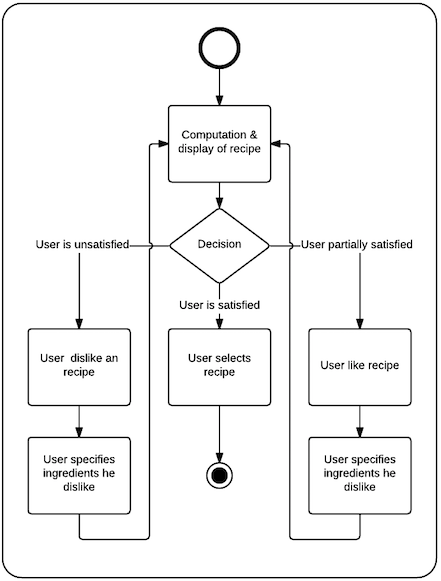
\includegraphics[width=.6\linewidth]{figures/ch3_critique_algo.png}
	  	\caption{FoodForMe Critiquing Algorithm.}
	  	\label{fig:ch3_critique_algo}
	  \end{figure}
	  
\newpage	  
\section{Persuasion}

Developing persuasive recommendation system (RS) is mainstream of this research. Traditionally, RS has been more focused towards algorithmic approaches and relied on them for providing accurate recommendations. As there was an assumption that the accuracy of algorithm is the key factor that affects the quality of recommendation. Recent studies shows there are other factors that plays a significant role in the acceptance of recommendation. Main factors are User-centric design for presenting recommendation, transparency of system (explain user how system works) via message and source. An other important factor that way influenced on acceptance is explanation of recommendation\cite{gkika2014persuasive}. In order to achieve Persuasion in our system we focus on   “Visualization or Presentation \cite{nanou2010effects} \cite{pu2006trust} and “Explanation of recommendation\cite{cialdini2009influence}\cite{fogg1998persuasive}”.
  
\subsection{Visualization or Presentation}

While investigating persuasion impact on recommendation our focus in terms of modality and organization of recommended items in order to achieve user satisfaction.  Hence, various recipe and food systems are compared in order to follow the social-orientation methodology, as it is part of user-centric approach and studies parameter that affects user preference and satisfaction \cite{ swearingen2002interaction}. After getting an idea about what are key factors in displaying recipes and what user expect form such system.  We structure our recommendations to increase the efficiency in selecting a recommended item and build trust and user satisfaction based on qualitative characteristics. Following are the approaches that we follow in organization of recommendations.

\begin{enumerate}
	\item Primary factors that consider while structuring recommendation item is user context to increase and maintain user interests in to the system to make system \textit{transparency and efficiency}. 
	
	\item Recommended item have recipe review count, rating and category and subcategory of recipe, recipe avatar, ordered by recipe title to achieve \textit{ effectiveness and satisfaction}
\end{enumerate}

\subsection{Explaination}

Although presentation and visualization will have an impact on persuasion but the key element in order to persuade something is the explanation about that recommended item. Any type of information additional information along with system’s output to achieve certain objective.  In our system our task is to persuade recipes, which suits according to user taste and heath preference. However, there is no clear indication in extant literature about what type of explanations can actually lead to persuasion and at what extend. Aim of providing the explanation to measure intensity of trust, credibility, satisfaction, accuracy and transparency of system. We started our research by finding the key element on which our explanation will depends by following Aristotle’s elements that helps in persuasion \cite{gkika2014persuasive}. Following are the explanation of each element with respect to our system. \textit{Ethos/Character of the speaker} refers to motivate user to cooking that recipe by getting the recipe for credible sources and convey message to user that our system cares him a lot by suggest him recipes according to his preferences. \textit{Message’s receiver pathos/emotions} Plays a vital role in persuading item. Health, taste and cooking preference are the primary consideration of user emotion. Our assumption was our system user are the diet conscious and want to live a better life. \textit{Logos/Argument} is reasoning why this particular recipe is given to him what are assumptions of system while considering this recipe. After finding out the key elements on which explanation is based on. Next step to apply the Cialdin’s Influence Principle\cite{cialdini2009influence} broadly used and verified for persuasion. Following are the description how we are applying each of the factor in our experiment.
  
  \begin{enumerate}
	\item \textit{Reciprocity} describes as humans have the tendency to return favors. In our system we are achieving the mechanism of rating of recipe. We assumed that by rating the recipe user is not only providing his feedback but also helps community in recipe selection. However, we also though about integrating user’s friends that will recommend him recipe based on his taste. Furthermore, we want to add dietitian that user can follow that will suggest him heath plan and based on that plan our system will recommend him recipe but this though is out of scope for this thesis.

	\item \textit{Scarcity} refers to people are inclined to consider more valuable whatever is scarce. In our system we implement this approach by the help of consumption context or categorizing the recipe according to consumption of recipe for instance breakfast’s recipes, juices etc. 
	
	\item \textit{Authority}  is implemented by the popularity of recipe among that course of recipe how much star it have and how user think about that  recipe.
	
	\item \textit{Liking} is implemented in two ways in our system. First by overall recipe rating and second is based on ingredients choices that are according to the taste of user.

	\item \textit{Commitment} is implemented by the considering the user preference. All recipes are that recommended to user have at least one of his favorite ingredient and his timing. Furthermore, we also mock exercise time to consume that recipe to keep focus on user’s health.
\end{enumerate}


Explanation of recommended item depends on: (1) How much calories are contained by recommended recipe (2) How much user needs to do exercise to burn such amount of calories. . (3) Factors why this particular recipe in user’s recommended item set. Let’s discuss each item hypothesis behind each of discuss item. Calories are important factor that person has to major if he wants to live healthier. To deal with health factor we have to provide calories information so that he can keep track of his consumption of calories. After given information about calories it is also important to highlight how much he have to workout to burn calories. Idea behind this to integrate app with another health or medical app and based on his health condition recommend him recipes. Moreover, it is also important to keep aware of user why system is recommending him such item. For this reason we consider user preferences about recipe and ingredients. More specifically every recipe which is recommended to user contains atleast one of his favorite ingredient. Additionally organized by cooking time which is provided by user according to his preference. Figure \ref{fig:ch3_explanation_generator} is a graphical representation how our system will generate recommendation’s explaination.

  \begin{figure}[h]
  	\centering
  	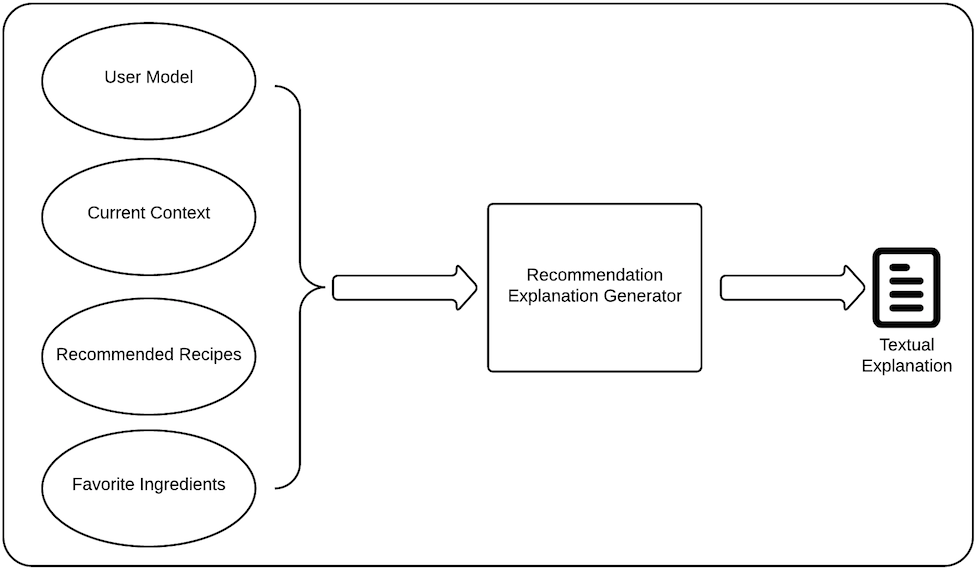
\includegraphics[width=.8\linewidth]{figures/ch3_explanation_generator.png}
  	\caption{Generation of recommendation explanations.}
  	\label{fig:ch3_explanation_generator}
  \end{figure}
\chapter{System Design and Implementation}

This chapter describes of the system. It starts by providing overview of the system, followed by requirement elicitation to build prototype. Furthermore, it also provide deeper understanding of architectural paradigm by discussing each module and their interconnection.

\section{Overview}

Pervious chapter limits our discussion about the design decision and describe the essential component of the system.  Since the concept is quite abstract and does not dictate any implementation details.  In order to challenge the relevance and capability of the concept, a prototype app, tailored to a real world scenario, should be developed as a “proof of concept”. Our system is divided in to two components: (1) Rest based web application follows modular principle of system design i.e. functionality of a system is divided into multiple concurrent modules. Where coordination of modules depend on database.  Each module has its own Data Access Object (DAO) through with communication take place. Module query existing data with the help of DAO perform their task and update afterward. (2) iOS client provides all the required interface to communicate with the server. It aims to collect information that needs to build user profile and allow active learning and critiquing mechanism to update user profile and increase the trust between user and system by conveying the idea how much system cares about user and his need. 

\section{Requirment elicitation}

This section represents user’s viewpoint of the system. It also describes the purpose of the system by identifying the Functional, non-functional requirements and description of use case in the form of scenarios. It is important to mention here that all the scenarios are developed to evaluate the prototype and are not meant for production purpose. 

\subsection{Functional Requirments}

FoodForMe is a mobile food recommender system that user iOS platform. It purpose to facilitate user to find the food what to cook that matches their personal preferences. Idea behind this prototype application is to proof the concept a combination of Persuasion and critique-based recommender system lead to better recommender and have an impact on user decision making process. Therefore all the functionality in a design is bounded to this purpose. There are two cases of interaction with the system. In case one user need login via Facebook so that system can get its demographic profile instead of asking him to fill out his personal information. Demographic information contains name, birthday, email, name and link of his profile picture. By default system keeps his cooking time preference and course selection preference. User can change these preferences from the setting screen. In second case user can interact without login and having same default preference. As it is notice that some user hesitate to provide their information without having a trust in a system. However, in this particular case user can only view the information. Our rest of discussion will relate do case one.\newline

After getting login and change his preference. User will able to view recipes according to his preference. Each recipe shows the name, star rating, main categories, sub categories, number of reviews and recipe picture. Once the user tap on any recipe, user is able to view detail of selected recipe. Detail screen consists on 3 to 4 sections depends on screen type. Section 1 contains the generic information about the recipe same as discuss above accept it provide large Image of recipe. In Section 2 is related to recipe ingredients, each ingredient item have its name and quantity. Section 3 is about preparation/direction means its guide user how to cook that recipe. Section 4 is an option selection and it will appear as per screen type. In this section system will provide why system think this recipe is according to user preference. User is able to see two screens that display recipes list. First one will display the popular recipes of the system. Recipe course and popularity are the factors on which this will depends on. Motivation behind this to aware user what’s new and hot in system and allow user to change his taste. On the other hand second list will depends only user preference. On detail screen of each recipe system will provide explanation, which tells user what system will think about him and why these recipe recommend to him. \newline

On the detail screen of selected recipe user can criticized on showed item. User can critique on list of indigents by mentioning them he like that ingredient or not. Also he might be able to critique on recipe by given star according to his choice. Additional system allow user to change his personal preferences these include cooking time and course selection. \new 


\subsection{Non Requirments}

From usability to performance aspect of a system Non-functional requirement can apply in many ways. However it is our assumption that this app is a prototype and will only use for evaluation purpose but we have to consider User interface, performance and supportable requirements. Following are some few non-functional requirements that should guide to development process:

\begin{enumerate}

		\item App must not be crash.
	\item Any mobile user can use the application and have a clear understanding of app without facing any problem.
	\item App should provide consistence user interface with respect to colors, fonts and theme.
	\item App should follow the Application User interface guideline provided by apple.
	\item For app start to critiquing or selection of preference must be reachable at any time.
	\item Processing time of app may not exceed to 1 second. 
	\item Server calls should not take more 30 sec.

\end{enumerate}

\section{System Architecture}

\subsection{Working}

\subsection{Class Drigram}

\subsection{ERD}

\section{System Services}

\subsection{Service 1}

\chapter{Evaluation}
Despite the fact, how good the prototype in terms of algorithmic and design approaches. There will be some probability that elaborates, users are doing what they are not expected to do.  This leads to other features(s) that needs to be develop in order to improves the user’s satisfaction and increase her willingness to user the system. Therefore it is important that developed system should go through an evaluation proves before it goes live. Focus of evolutions to ensure that product is appropriate and the involvement of user through the design process. This chapter depicts the evaluation of prototype in a real user study and present the result.
\section{Motivation and Goals}
Motivation behind performing evaluation to determine, whether the process of recipe according to user interest in mobile critique-based recommender system can be improved by applying Persuasive Principles. As discussed earlier, purpose of developed Food Recommender System aim to be used in a real world situation. This established some aspects of the user study, including the development of a variant of the proposed application and assessment of the system.\newline
During the study, two variants of the system will need to be tested, one begin the basic interface design, without explanation and works on basic recommender system by providing star rating to the recipes. Whereas, the second system is the main output of thesis, with better infrastructure of recipes, sleeker interface and having explanation about the recipes. Additionally recommender system algorithm supports critiquing on both ingredients and recipes.\newline 
The study is designed in a way that each user has to test both variants of the application, which system is more appealing for the users. Focusing on real effect of recommendation depends on factors like user intent, context, way to present recommendations set and other. Thus experiment needs to provide evidence as the true value of evaluation.\cite{shani2011evaluating}. Additionally a single irritation of user study should not exceed with more then 20 min to maintain user interest. Considering the fact that user have to test two variant of application. However it is possible that user might have get some less qualitative results which is not due the fault from the system but because users were overwhelmed with long sessions.  \newline
The focus of evaluation was to measure the effect of persuasion by providing the recommendation in form of recipes. Also how active learning also system to change itself according to user preferences. However it exclude the non-relevant part like ingredients integration to improve the recipes.
\section{Data set Generation}
Data sets are necessary to create a pragmatic setup to represent a real world objects. Therefore, a data crawler needs to be developed as an open-source project that will crawl the recipes form any recipe data bank. Crawler developed by us is written in java.  Crawling recipe form data bank is a two steps process.  First fetches the recipes from databank on behave of food type and course.  In second step it will sync all those recipes whose details are not present in our database. Additionally recipes images are not been stored in our system instead of saving image we stores their URLs. Extracted data provide international recipes of different cousins. However, it provides functionally to add more different data source that provides recipes. To keep the amount of work reasonable items were associated with the following:
\begin{enumerate}
	\item Unique identifier for recipes
	\item 11 types of courses (e.g,. Appetizers, Bread)
	\item 91 Cuisine (e.g. American, Thai, Beverages)
	\item Images links of different sizes
	\item Preparation
	\item List of ingredients
	\item Popularity of recipe
\end{enumerate}
Currently our data bank has 1303 of recipes, 10037 ingredients. Furthermore, it can grow more depends on crawling method.
\section{Setup}
This section leads our discussion toward the selection of test hardware, different variants of application and testing framework for the sake of performing evaluation.
\subsection{Test Hardware}
Recommended hardware must have at least 320x 480 resolution and above, running iOS version 8.0 or later. In order words required device to run application is iPhone 4S and above.  
\subsection{Variants}
Two variants of system are developed to test. Both variants use the same recommendation algorithm. However they are different to each other by have unique interface design, explanation of recommendation and critiquing methodology.
\subsubsection{Experiment (EXP)} 
This variant refers to the proposed developed system as discuss in chapter 4. It allows users to change their preferences while interacting to the system by critiquing on ingredients and recipes. System provides explanation to each recommended item. Additionally interface follows the user centric design, which contains more information about the recipe to draw user attention towards recipes.
	
	\subsubsection{Basic (BASE)}
Consider as baseline to compared the needs and effectiveness of actual system. EXP is the extension BASE.  Both variants (BASE and EXP) share the same app but have different interfaces, from app main menu users can select which system they would like to use. Amount of information provided by BASE is similar to existing apps that are currently available in market. To display a recipe the content that is considered by the system are recipe title, recipe avatar (indicates how does it look), ingredients, preparation method and star rating that shows the popularity of recipe. It presents the recipes in a list fashion, on tapping on a recipe detail screen open. User can critique on recipe by tapping on critique button at the top right corner presented on recipe detail screen.  Besides providing recipe avatar all the information provided by BASE is textual form. It does not provide explanation to user why this recipe recommends to her, not indicates the factors that system consider while making a recommendation. Also user can critique on a recipe by giving stars. Figure \ref{fig:foodforme_base_recpie} represents it's user-interface. 

	  \begin{figure}[h]
	  	\begin{subfigure}{.32\textwidth}
	  		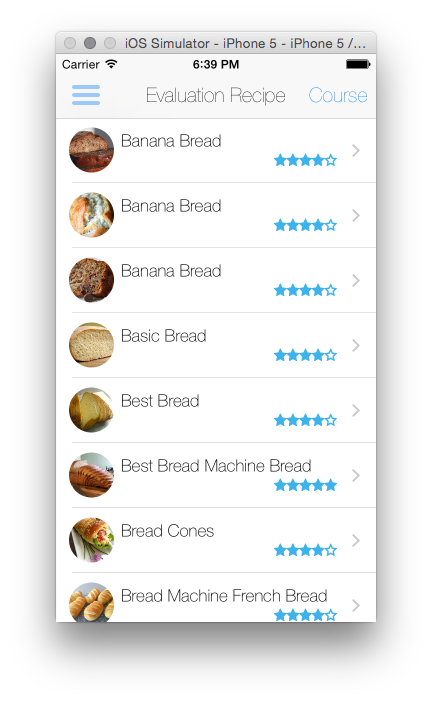
\includegraphics[width=.9\linewidth]{figures/ch4_app_screen_shots/test_system/evaluation_recipe}
	  		\caption{Recipe}
	  	\end{subfigure}
	  	\begin{subfigure}{.32\textwidth}
	  		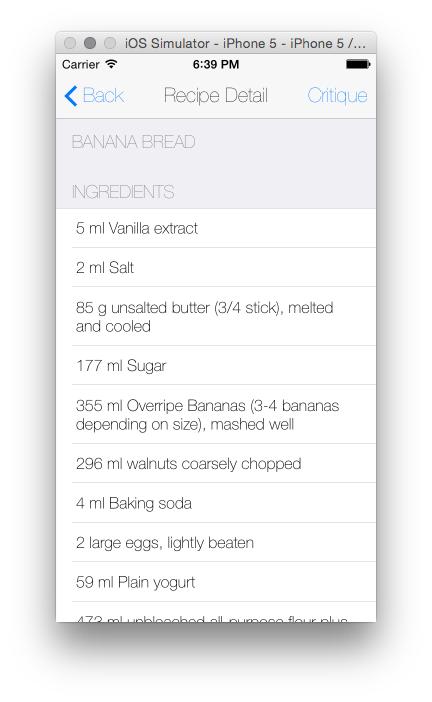
\includegraphics[width=.9\linewidth]{figures/ch4_app_screen_shots/test_system/evaluation_recipe_detail}
	  		\caption{Recipe Detail}
	  	\end{subfigure}
	  	\begin{subfigure}{.32\textwidth}
	  		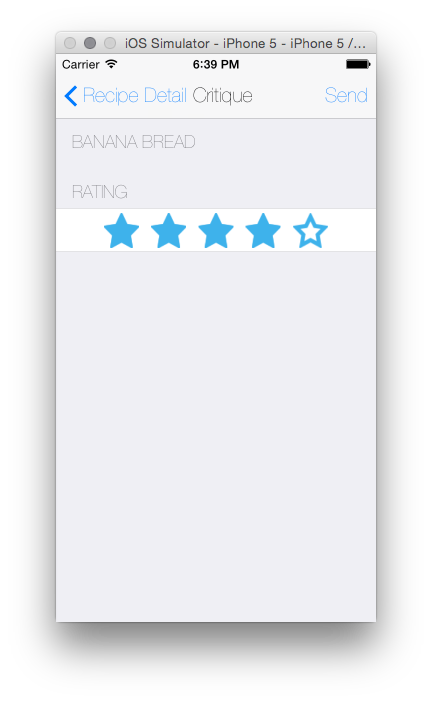
\includegraphics[width=.9\linewidth]{figures/ch4_app_screen_shots/test_system/crtiquing_evaluation_sysetm}
	  		\caption{Recipe's Critique}
	  	\end{subfigure}
	  	\caption{FoodForMe BASE Recipe}
	  	\label{fig:foodforme_base_recpie}
	  \end{figure}
\newpage
\subsection{Testing Framework}
Testing framework that is applied in user study is a subset of the aspect that are relevant for persuasion and critiquing in recommend system. It follows the user-centric design approaches \cite{pu2006trust} and framework that applied for evaluation of recommend recommendation system \cite{shani2011evaluating}. Measure data is divided into following areas:
\subsubsection{Persuasion’s Principle}
Persuasion’s principle that discussed in section \ref{ch4_persuasion_explaination} were related to the how these factors will be implemented in our system.  It is essential aspect for this thesis that the recommendations that are suggested to user should ne persuasive in nature and follows the principle. The forth-coming discussion relates whether user might be able to perceive those or not.
  \begin{enumerate}
  	\item \textit{Perceived Reciprocity} is allows user to return her favor by critiquing as recipe and select other good food according to particular food course and cuisine. The participants were asked they think that system helps them to select them a recipe although this recipe is according to her preferences, but the system consider other user feedback on that recipes before making up recommendations.
  	
  	\item \textit{Perceived Scarcity} measurement indicates by categorizing recommendation with respect to context and consumption time of recipe. Participants were asked whether they find that system helps them to filter out the recipe according to their meal time.      
  	\item \textit{Perceived Authority} refers to the popularity of a particular recipe in a given context of user. To measure the level of perceived authority, Participants were asked to what ascent they felt authority. 
  	
  	\item \textit{Perceived Liking} refers to factors that include liking a recipe. In our system measure matric was based on ingredients and recipe staring. Participants were asked which mechanism like/dislike help more in finding out the recipe. 	  
  	
  	\item \textit{Perceived Commitment} indicated to what degree system is committed to user preference. In order to measure the degree of commitment metric is defined. Participants were asked to mark if they felt that system is committed to preferences or not.	  
  	  	
  	\item \textit{Perceived Social Proof} denotes the what society think about that particular item in our case recipe. User may or may not thought that social factor is present, By asking the user to what level they consider social factor is present in our system by providing them a scale.   
  \end{enumerate}
  
\subsubsection{Transparency}
Ability of a system that allows user to understand its working and explain system choices and behavior. However it is possible that user’s understanding about the system working might be differ form its actual working. For the sake of evaluation user were asked to mark choices that they think about the system when making recommendations. \newline
\textit{Perceived Transparency:} There is a possibility that user might or not perceive that system is transparent. By asking the factors which users thinks system include while making a recommendation. It is possible learn their perceived transparency.

\subsubsection{User Control}
Level of control that provides to users while operation a system refers to User Control. Under this sub section we want to measure the following items:  \newline
\textit{Perceived Overall Control} indicates that does user have overall control over recommendation. The participant were asked about what they feel about while using the application by rating that were they able to tell about the system which recipes are the looking for, telling their preference to system and finally to what assent they feel they have control over system. \newline
\textit{Perceived Scrutability} denotes the ability of the system that allows user to revised their preference and excludes those assumptions that system made on there behaves. Participants were asked to rate till what ascent they feel control over system to correct the wrong assumption made by the system.
\subsubsection{Efficiency}
Providing good recommendation is not only the task of recommender systems. Also it is essential for a system how quickly it come to decisions that help in selection of item especially in the domain of mobiles. Measuring efficiency is divided into two perspectives. First, as in conversational recommender numbers of cycles were counter.  Where each cycle defined as number of times user have to perform update his/her preference in order to complete a task. Each cycle have an impact on user model. Second refers as time that passed from display of first recommendation set to selection and confirmation of required item. Where time measure in seconds.\newline
\textit{Perceived Efficiency} Duration of item until item found is hard to perceive for user. Therefore for the sake of simplicity user were asked if it requires to much effort to find a recipe they are looking for. Additionally run of cycles are also hard to reminder but since conversation system cycle normally cycle are not be exceed to two cycle. Therefore user were asked to mention in which cycle they received their recipe. 
\subsubsection{Satisfaction}
Satisfaction is the ability to make system fun while user is interacting with the system. Also providing poor recommendation decrease the user interest.\newline
\textit{Perceived Satisfaction} measure to determine user’s feeling while in using system. It allows user to express their preferences about the system in a direct way. Participants were asked to which ascent they were satisfied about they system.
\subsubsection{Context}
Context defines as any information that can be used to characterize the situation of entity. It is important for recommendation to consider the context while making a recommendation in order to make the recommendation more concrete. \newline
\textit{Perceived Context} are determine in following ways: calories information about the recipe, cooking time and course of recipes. Participants were asked to select which contextual information helped them to select to recipe. 
\subsubsection{UserDemographic}
Participants were asked to fill their demographic information for instance age, occupation, how often they cooked. 
\subsection {Testing Procedure}
Evaluation's testing procedure was structured in the following order:
 \begin{enumerate}
 	
 	\item  Initially participants were asked to provide their background information, which include age, occupation. Additionally they need to provide how often they cooked considered demographic information.
 	
 	\item Next step was to present the idea of system and the purpose of user study to the participant. So they have a clear understanding about both presented items.  
 	
 	\item Instead of requesting user to pick up the random recipe according to their interest present a realistic scenario, which helps user in order to mention their interest like as follows:\newline 
 	
 	\textit{Imagine you just came for gym. You need prepare a meal for yourself. You have prepared a meal according to you taste and diet plan and have an hour for cooking.  You are not sure what to cook. You opened FoodForMe app and start looking what needs to prepare. After you find the recipe you need to provide your feedback.}\newline
 	\textit{For first step your task is:}\newline
 	\textit{Find a recipe you would lie to cook if given the opportunity that satisfies the following:}
 	\begin{enumerate}
	 	\item \textit{Cooking time 90min.}
	 	\item \textit{Type of recipe : Appetizer,  bread, breakfast, salads, soups etc.}
 	\end{enumerate}
 	\textit{After introducing task, hand over the app to users so that familiarize themselves with the interface and app workflow. They were also asked that this task would be executed twice with two different variants of the app, leading to potentially better or worse recommendations. Finally they need to judge which variant is better.}
 	
 	\item After demonstration of task, users need to understand how to perform critique and setup their preferences. 
 	
 	\item Participants were encouraged to given their verbal feedback about the system. Although it'ss not mandatory. All the verbal feedbacks were noted. 
 	
 	\item Once the tester performed his/her task and selects the recipe, which is satisfied as per his/her preference. The whole process was repeated for other variant of the system. 
	\item Finally each participant was interviewed about which  variant they liked the most and why by filing a questioner. 
 \end{enumerate}
 
\section{Results}
In this section our discussion leads to the result of data points measures via user study.  

\subsection {Participants}

	  \begin{figure}[h]
	  	\centering
	  	\begin{subfigure}{ .70\textwidth}
	  		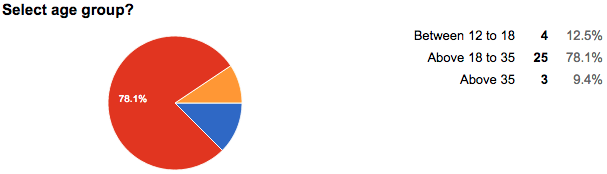
\includegraphics[width= 1\linewidth]{figures/ch5_stat_age.png}
	  		\caption{Participants Age}
	  
	  			\end{subfigure}
	  
	  		\begin{subfigure}{.70\textwidth}
	  		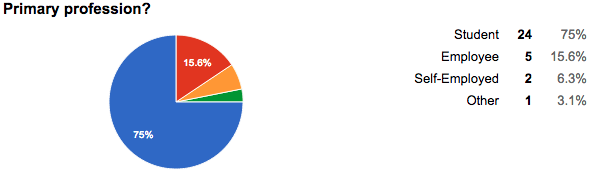
\includegraphics[width= 1\linewidth]{figures/ch5_stat_profession.png}
	  		\caption{Participants Profession}
	  	\end{subfigure}
	  	\begin{subfigure}{.70\textwidth}
	  		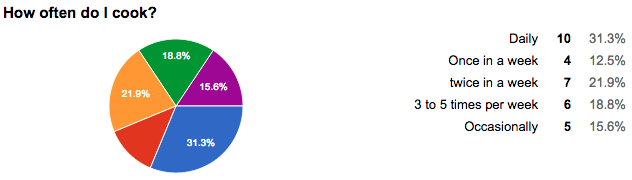
\includegraphics[width= 1\linewidth]{figures/ch5_stat_cook.png}
	  		\caption{How much Participants cook}
	  	\end{subfigure}
	  	\caption{Participants Demographic Info}
	  	\label{fig:stat_demographic_info}
	  \end{figure}
	  
People who performed evaluation was belong to various age groups and have different occupation. Overall 31 people participated, 24 students, 5 employee, 2 self-employed and 1 is housewife. 78.1\% of them have age between 18 to 35 years.  12.5\% are between 12 to 18 years old. Where people whose ages are above 35 year have a small portion, which is 9.4\%. However mostly participants like to cook on daily bases. In addition to this 21\% of participants cook twice a week and 18.8\% said that they need to cook 3 to 5 timer per week and rest are those how cook occasionally. Figure \ref{fig:stat_demographic_info} shows their distribution in terms of age, cooking preferences and professional separately.

\subsection{Perceived Persuasion}
Significant change in user’s intension to cook a recipe has been observed form the result. To determine which strategies preform better in terms of persuasiveness, paired t-test were used upon the difference between initial rating and the one for each strategy. The results in Table \ref{table:persusasion-result} reflects the effectiveness comparison among the strategies. 
\begin{table}[ht]
	\centering % used for centering table
		\begin{tabular}{p{2cm} p{2cm} p{2cm} p{2cm} p{2cm} p{2cm}}
		\hline\hline 
			%inserts double horizontal lines
	
				& Scarcity & Authority & Social Proof & Liking & Commitment\\ % inserts table
		%heading
		\hline % inserts single horizontal line
				Reciprocity   & <0.001  & <0.001 & <0.001 &  0.083 & <0.001 \\ % inserting body of the table
		
		Scarcity      &         & <0.001 &  0.169 & <0.001 & <0.001 \\
		
		Authority     &         &        &  0.089 & <0.001 &  0.325 \\
		
		Social Proof  &         &        &        & <0.001 &  0.083 \\
		
		Liking        &         &        &        &        & <0.001 \\
		
		Commitment    &         &        &        &        &  \\ [1ex] % [1ex] adds vertical space
		\hline %inserts single line
			\end{tabular}
				\caption{Paired t-test was used to examine significance, where 0.05 is set as the threshold for p-value to evaluate the significance and p-value lower than 0.001 indicates strong significance.}
				\label{table:persusasion-result}

\end{table}

Next we discuss the impact of each of the persuasiveness factor individually and focus on what was the consideration of participant about them.\newline
\subsubsection{Reciprocity}
Selecting which system is most like by user does measurement of Reciprocity. System that provides only textual information was BASE and on the other hand EXP has more information contains all the graphical information about recipes. People are more reluctant towards EXP i.e. 93.8\%. Figure \ref{fig:ch5_stat_reciprocity} represents the reciprocity measurement.
\begin{figure}[h]
	\centering
	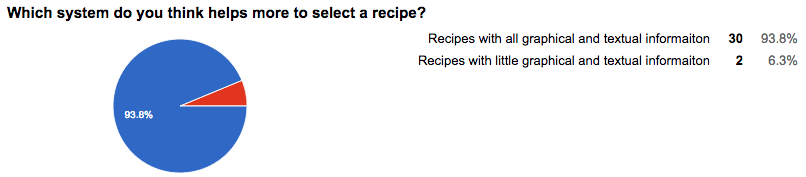
\includegraphics[width=1\linewidth]{figures/ch5_stat_reciprocity}
	\caption{Perceived Reciprocity}
	\label{fig:ch5_stat_reciprocity}
\end{figure}
\newpage
\subsubsection{Scarcity}
Asking the participants what they feel about scarcity by filtering out the recipe with respect to meal by provide the liker scale. Where 1 mean strongly agree and 5 means strongly disagree.  34.3\% of them were quite sure about it and 43.8\% feel good about that. Additionally 15.6\% were moderate about this statement. Where 6.2\% how felt negative about this statement. 
\begin{figure}[h]
	\centering
	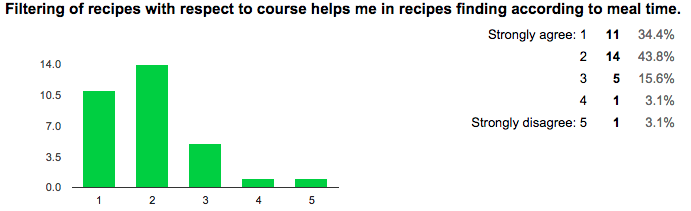
\includegraphics[width=1\linewidth]{figures/ch5_stat_scarcity.png}
	\caption{Perceived Scarcity}
	\label{fig:ch5_stat_scarcity}
\end{figure}
\subsubsection{Authority}
Measuring the authority by asking liker scale question, did they feel that recipe star rating help them in selection of recipe. 93.8\% of participants were positive about that. Conversely people how negate that statement were 6.2\%. Figure\ref{fig:ch5_stat_authority} represents overall statics. 
\begin{figure}[h]
	\centering
	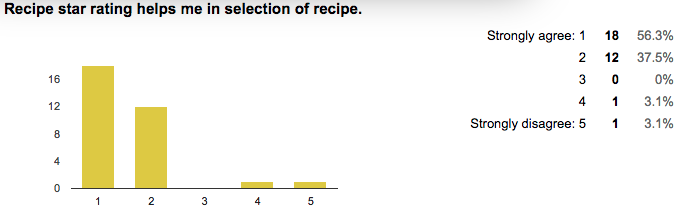
\includegraphics[width=1\linewidth]{figures/ch5_stat_authority}
	\caption{Perceived Authority}
	\label{fig:ch5_stat_authority}
\end{figure}
\subsubsection{Liking}
When ask the participants which recipe critiquing technique helps them in finding their recipe. Majority of them voted for critiquing on both ingredients and recipe which in 78.1\%. On the hand minor portion of the participant i.e. 21.9\% liked the conventional critiquing technique to provide their feedback.
\begin{figure}[h]
	\centering
	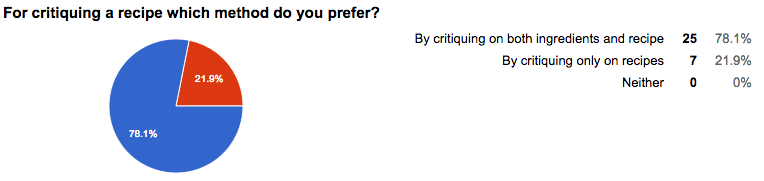
\includegraphics[width=1\linewidth]{figures/ch5_stat_liking.png}
	\caption{Perceived Liking}
	\label{fig:ch5_stat_liking}
\end{figure}
\subsubsection{Commitment}
Participants considered the commitment by providing their answers to liker scale question. In which they have to mention, do they feel explanation of recipe helped them in recipe selection. 90.7\% believed in that statement. Conversely, minor amount of dined to the statement. Where as only 3.1\% were neither agree nether dined to the statement. Figure \ref{fig:ch5_commitment} shows the feedback.
\begin{figure}[h]
	\centering
	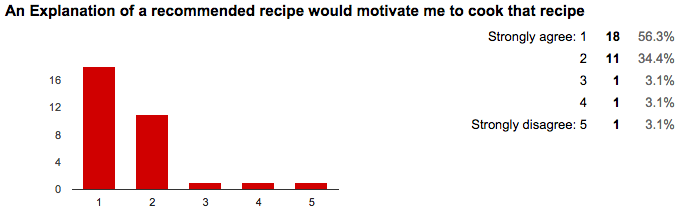
\includegraphics[width=1\linewidth]{figures/ch5_stat_commitment}
	\caption{Perceived Commitment}
	\label{fig:ch5_commitment}
\end{figure}
\subsubsection{Social Proof}
Social proof was measured by asking a likert scale question. In which they had to answered whether participant agreed that he understand that rating a recipe not only helps him to receive better recommendations but also the whole community. 84.4\% of participant were positive and endorsed this fact. In contrast to that a small spike in Figure \ref{fig:ch5_stat_social_proof} represents to those 12.5\% participants how were not favor to that. 
\begin{figure}[h]
\centering
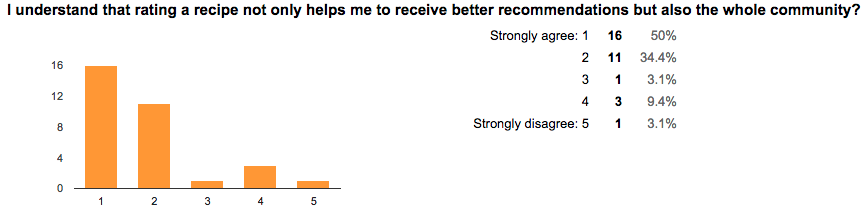
\includegraphics[width=1\linewidth]{figures/ch5_stat_social_proof.png}
\caption{Perceived Social Proof}
\label{fig:ch5_stat_social_proof}
\end{figure}
\subsection{Perceived Transparency}
Once the user performs their task they were asked about how the underlying recommendation system variants work to measure transparency effect. In general, the percipients were able to explain that based on their preferences system builds a there model in each cycle and generate a recommendation for them.  While observing the result there is no clear distinction between the variants. In general, participants felt EXP is more transparent then BASE.  Mean average of EXP is 4.344 compared to the BASE which is 4.125. While analyzing the standard deviation EXP ${\sigma}$ = 0.7007 and BASE ${\sigma}$ = 0.7931. Further analysis suggested that EXP that provides explanation perceived to more transparent (one-tail t-test, p<0.05 with p= 6.06E-03). Figure \ref{fig:ch5_stat_transpancy} shows the rating distribution between two variants. It can be seen clear that in EXP people are more satisfied with respect to BAES. Although there are some participants how feel that system is complex.
\begin{figure}[h]
	\centering
	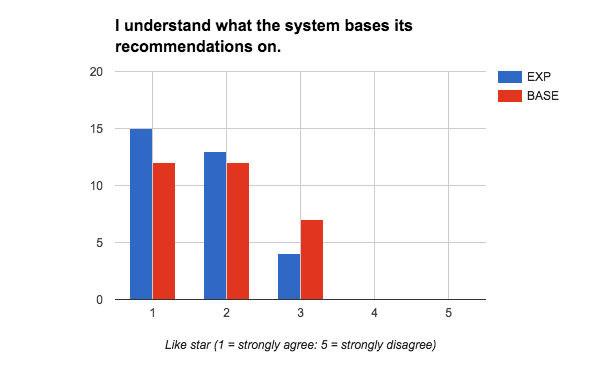
\includegraphics[width=1\linewidth]{figures/ch5_stat_transpancy.png}
	\caption{Perceived Transparency}
	\label{fig:ch5_stat_transpancy}
\end{figure}
\subsection{Perceived User Control}
In our earlier discussion in this chapter, to measure the effect of user control we divided into overall control and suitability perceived by user. 
\subsubsection{Overall Control}
To observe that user were able to perceived overall control or not. They asked about did they felt control while telling the system what they want.  Mean average of EXP is 4.219 where BASE = 3.219. Standard deviation of EXP ${\sigma}$ = 0.8701 and BASE ${\sigma}$ = 0.9750. Also further analysis proves that EXP seems to be significantly better than BASE (one-tail t-test, p> 0.05 with p = 2.31E-12). Figure \ref{fig:ch5_stat_overall_control} reflects the actual distribution of rating. Where EXP has 87.5\% over positive rating, where there are some percentage of people feel neutral about system where 3.1\% doesn’t feel control.
\begin{figure}[h]
	\centering
	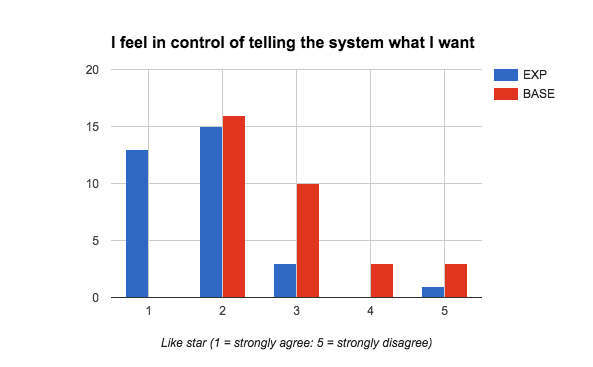
\includegraphics[width= 1\linewidth]{figures/ch5_stat_overall_control}
	\caption{Perceived Overall Control}
	\label{fig:ch5_stat_overall_control}
\end{figure}
\subsubsection{Scrutability}
Scrutability measured by asking the user did they feel ease of correcting mistake made by system. EXP performs a lot better than BASE. Mean average of EXP = 4.000 and BASE 2.313. Consider Standard deviation EXP ${\sigma}$ = 0.9504 and BASE ${\sigma}$ = 0.9651. On more analysis result also support that Scrutability is perceived on EXP than BASE.(One-tail t-test, p<0.05 with p = 1.91E-19
). Actual distribution of rating in Figure \ref{fig:ch5_stat_scrutability} reveals the significance of EXP over BASE.
\begin{figure}[h]
	\centering
	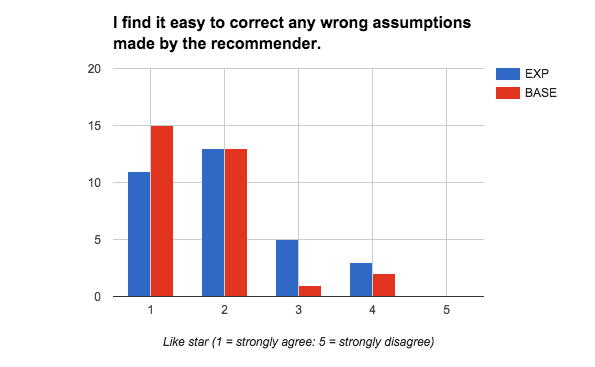
\includegraphics[width= 1\linewidth]{figures/ch5_stat_scrutability}
	\caption{Perceived Scrutability}
	\label{fig:ch5_stat_scrutability}
\end{figure}
\newpage
\subsection{Efficiency}
Efficiency is measured by analyzing the number of critiquing cycle (number of user updates to the preferences by the mean of critiquing). 
\subsubsection{Cycles}
Participants were asked to mention in which cycle they felt they had received their item.  On average participants completed their task in min 3 cycles before.  EXP mean average = 3.625
 and BASE  = 7.000 where standard deviation of EXP ${\sigma}$ = 0.8328 and BASE ${\sigma}$ = 1.1914. However one-tail t-test suggested that EXP is more significant than BASE( p< 0.05 with p =  4.21E-23). Figure \ref{fig:ch5_stat_efficiency_cycles} illustrates the number of cycles that users had performed to complete their task. 
\begin{figure}[h]
	\centering
	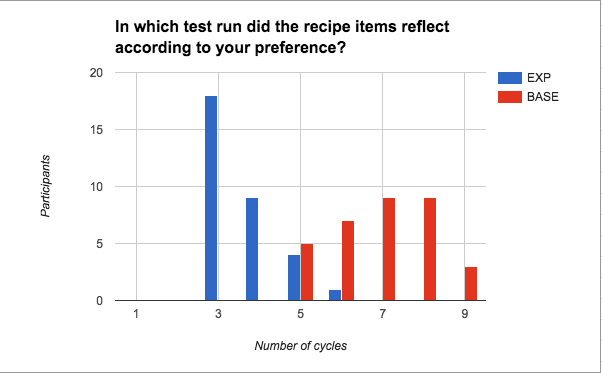
\includegraphics[width= 1\linewidth]{figures/ch5_stat_efficiency_cycles}
	\caption{Number of cycles}
	\label{fig:ch5_stat_efficiency_cycles}
\end{figure}
\newpage
\subsubsection{Perceived Efficiency}
Participants were asked about whether they felt that find the recipe requires too much effort for them. The participants felt satisfaction about the EXP. Average rating got by EXP = 1.844 and BASE = 2.500. Consider Standard deviation EXP ${\sigma}$ = 0.6278 and BASE ${\sigma}$ = 1.1359. One-tail t-test result also in the favor of EMP where p <0.05 with p = 9.13E-06. Figure \ref{fig:ch5_stat_effiiciency} reflects the user choice how they perceived the efficacy in both systems.
\begin{figure}[h]
	\centering
	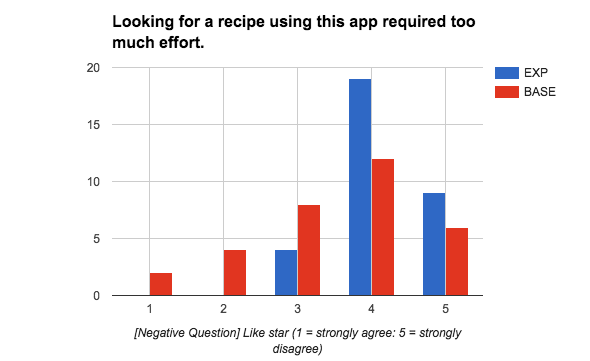
\includegraphics[width= 1\linewidth]{figures/ch5_stat_effiiciency}
	\caption{Perceived Efficiency}
	\label{fig:ch5_stat_effiiciency}
\end{figure}
\newpage
\subsection{Perceived Satisfaction}
Satisfaction is measures by inquiring users about their though while interacting with the systems. EXP have better results then EXP by having average of 4.313 against 2.469. While  Standard deviation EXP ${\sigma}$ = 0.8958 and BASE ${\sigma}$ = 0.9153. By looking at one-tail t-test result we conclude that results are significant (p< 0.05 with p=4.50E-16). Analyzing the rating distribution in Figure \ref{fig:ch5_stat_satisfaction} make it more clear. 
\begin{figure}[h]
	\centering
	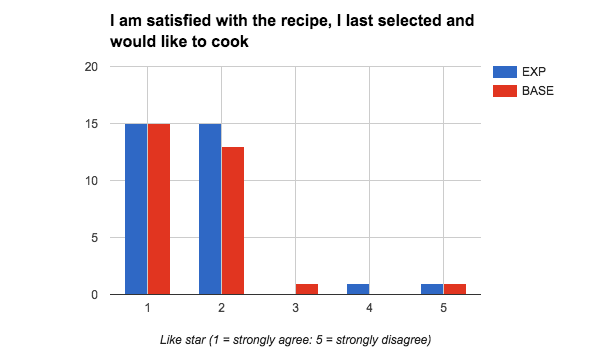
\includegraphics[width= 1\linewidth]{figures/ch5_stat_satisfaction}
	\caption{Perceived Satisfaction}
	\label{fig:ch5_stat_satisfaction}
\end{figure}
\newpage
\subsection{Perceived Context}
Participants were asked which contextual information they considered more while selecting a recipe according to preferences. Contextual factors are categories in two major section Calories information, which further divided calories, contains by recipe itself and amount of exercise need to bee done to burn such calories. On the hand context like cooking time and course of the recipe are consider. Considering the result showing in Figure \ref{fig:ch5_stat_context} participants that consider calories information in their diet are 75\% which is majority of population. While more then half population of participant considers recipe course and preparation of recipe. 
\begin{figure}[h]
	\centering
	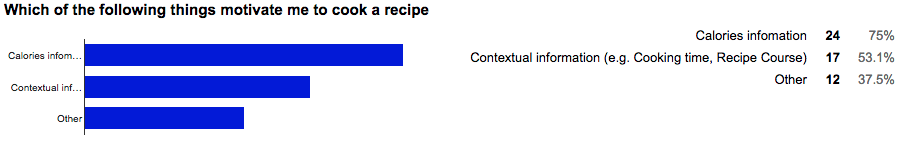
\includegraphics[width= 1\linewidth]{figures/ch5_stat_context}
	\caption{Perceived Context}
	\label{fig:ch5_stat_context}
\end{figure}
\subsection{Informal Feedback}
Our user study was not about feeling questionnaire, Informal feedback given by participant were also encourage and considered as valuable. It is important mention that each feedback was taken separately to each user based on their experience with other apps. Mainly user feedback were around what they feel are missing in our system and existing once. However it fairly possible that other may disagree with these options. Our discussion in this section focuses on most mentioned and participant’s interest feedback. \newline
\subsubsection{Explanation Enhancements}
 	\begin{itemize}
 		\item Some participants mentioned that it would be more helpful for them if the context in a explanation are highlight. It will allow them to take a decision without closely reading the whole paragraph.
 		
 		\item  While some people think that it would be great if explanation of tells recipe us about how does it taste for instances bitter, spicy, mild. 
 		
 		 \item Additionally, fewer people said that it would be nice to have origin of recipe in explanation part. Although it has been shown on top header but considered this section, they accept all the information about the recipe. 
 	\end{itemize}
 	
\subsubsection{More Attributes}
	\begin{itemize}
		\item Majority of participants suggested after seeing calories information in explanation section, they would love to have a feature that would keep track of deity information by allowing them to set a target like how much they want to put on or lose weight.
		 
		 \item Some participant added the above clause by suggesting that there should be a mechanism that will recommend us a weekly diet plan.
		 
		 \item Fewer participants were raised thought that app should consider also what ingredient they have and what recipes they can cook along with that items. 
		\item In addition to above point 1 or 2 participants suggested idea the app will attract them more if they can edit a recipe and contribute their recipes to the system. 
	\end{itemize}
\subsubsection{Endless set of recommenadations}
Quite few users reported, instead of given them specific amount recipes it would be quit helpful if app should provide a pagination functionality so that they can scroll and are able to more and more recipes. By providing us examples of some available products.
	
\subsubsection{Allow sorting}
Fewer participants felt that the app should allow them a functionality to sort the recipes according to type for example, sorting based on popularity and reviews.\newline
Finally, it was observed that as if there are so many ingredients that are liked by users, he can get much or more specific result with critiquing again, that he or she looking for because of limit amount of item set. To solve this problem user should provided endless recommendation set.
\subsection{User Preferences}
Last part of evolution was to ask the participant which variant they liked most why. More then 90\% of participants were in the favor of EXP over BASE. Reasons were BASE has allowed them to critique only the recipes because of this critiquing cycles were increased to 2X to 3X. Furthermore, participants liked to know what the system thinks about their preference and why this recommendation is for them EXP allows them where BASE don’t. Last but no the least only providing the recipes details is not sufficient for user, People want more and more information about the item which they select the more information they have the better they previse. 
	  \begin{figure}[h]
	  	\centering
	  	\begin{subfigure}{.80\textwidth}
	  		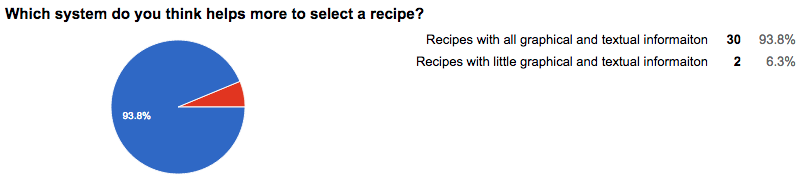
\includegraphics[width=.9\linewidth]{figures/ch5_stat_user_preference_recipe_info}
	  		\caption{Recipe Information}
	  	\end{subfigure}
	  	\begin{subfigure}{.80\textwidth}
	  		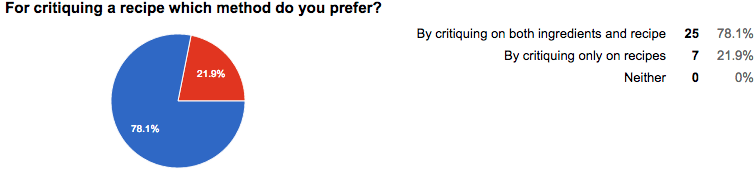
\includegraphics[width=.9\linewidth]{figures/ch5_stat_user_preference_recipe_critique}
	  		\caption{Recipe Critique}
	  	\end{subfigure}
	  	\begin{subfigure}{.80\textwidth}
	  		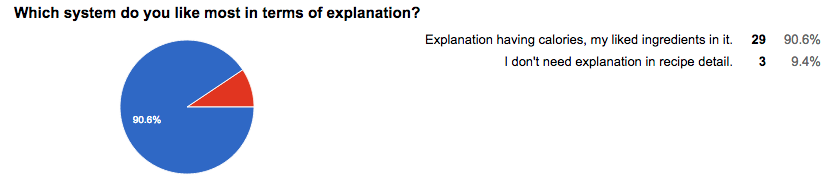
\includegraphics[width=.9\linewidth]{figures/ch5_stat_user_preference_recipe_explanation}
	  		\caption{Explanation}
	  	\end{subfigure}
	  	\caption{User Preferences}
	  	\label{fig:ch5_stat_user_preference}
	  \end{figure}
	  
\section{Discussion}
After elaborating on the measurements, now each point will be further analyzed to explain the observed results and share the lessons learned for future improvements. \newline
Starting our discussion with persuasion, EXP has more positive feedback compared to BASE. As per results 90\% of participants in the favor of EXP. Let’s narrow down the discussion to each Principe of Persuasion.  EXP achieved more then 93\%\ of \textit{Reciprocity} than BASE. Participant thinks that preferred information that requires selecting a recipe should contains other review about the recipes and user-centric approach, which involved all textual and graphical information about the recipes.  Overall \textit{Scarcity} is achieved by the system s 78.8\% by filtering out the recipes with respect to consumption time. \textit{Authority} is perceived by 93.8\%, participants feel star rating helps them in recipe selection. \textit{Liking} 78.1\% people in the favor of EXP which means they want to critique on recipe as well as ingredients. EXP leads BASE in terms \textit{Commitment}, 90.7\% of user thought that explanation of recipe motivate them to cook the recipe. Lastly, 
\textit{Social Proof} achieves 84.4\%. Overall looking into the result, we can draw our conclusion that EXP is far more persuasive then BASE. However in order to system more persuasive system should consider more health factors. \newline
In terms of transparency, both system performs well there is no clear winner. Considering the fact system is simpler when it allows small number of items to critique on. However by looking into the results of conducted serve, mostly participant were able to tell the system’s behavior. Moreover, EXP seemed to be transparent to participants, because it provides an explanation. In this case we can draw a conclusion that EXP is superior than BASE. \newline
User felt more control over EXP because it provides explanation through which user could grab an idea what factors are involved in making this recommendation. In addition to EXP allows user to correct the wrong assumption that has been made by the system, which relates to the goal scrutablility. While in BASE it was pretty hard to correct the wrong assumption since it dealt which overall weight of the recipes. \newline
Efficiency has been observed in two ways number of critique cycle that user need to perform to get the particular recipe and overall efficiency of the system in which we measured how much efforts required for a user to find a recipe. In terms of number of cycles EXP provide more efficient result in shorter number of cycle than BASE. Since the critiquing criteria followed by BASE is easy but lead to large number of cycle. Where as intuitive critiquing design of EXP allow users to critique on recipes as well as ingredients which lead to shorter critiquing cycle and far better result then BASE. However people find system is efficient in both variant in finding recipes but comfortable in EXP more than BASE. This might due explanation and over all improved design. \newline
Level of satisfaction of EXP user is remarkably higher than BASE. Although both variants got the positive feedback but due to slick and user-centric design of EXP, its immediately captures the user attention.\newline

Considering the contextual information about the recipe. It seemed like people are more focus towards that system which include calories information along with cooking time and course selection. BASE has got 53.1\% of positive comment but EXP wins again by gain 23\% more votes then BASE. Overall votes for EXP were 75\%.  
Overall, participant prefers EXP over BASE and found more persuasive in nature. Users were comfortable about the explanation about the system and want some more information in it. They found system transparent, efficient, satisfied and provide significant control to them. However, to make system more appealing some changes need to be implemented which includes, consideration of health, sorting, pagination in recommendation list.  
\chapter{Evaluation And Conclusion}

Despite the fact, how good the prototype in terms of algorithmic and design approaches. There will be some probability that elaborates, users are doing what they are not expected to do.  This leads to other features(s) that needs to be develop in order to improves the user’s satisfaction and increase his willingness to user the system. Therefore it is important that developed system should go through an evaluation proves before it goes live. Focus of evolutions to ensure that product is appropriate and the involvement of user through the design process. This chapter depicts the evaluation of prototype in a real user study and present the result.

\section{Motivation and Goals}

Motivation behind performing evaluation to determine, whether the process of recipe according to user interest in mobile critique-based recommender system can be improved by applying Persuasive Principles. As discussed earlier, purpose of developed Food Recommender System aim to be used in a real world situation. This established some aspects of the user study, including the development of a variant of the proposed application and assessment of the system.\newline

During the study, two variants of the system will need to be tested, one begin the basic interface design, without explanation and works on basic recommender system by providing star rating to the recipes. Whereas, the second system is the main output of thesis, with better infrastructure of recipes, sleeker interface and having explanation about the recipes. Additionally recommender system algorithm supports critiquing on both ingredients and recipes.\newline 

The study is designed in a way that each user has to test both variants of the application, which system is more appealing for the users. Focusing on real effect of recommendation depends on factors like user intent, context, way to present recommendations set and other. Thus experiment needs to provide evidence as the true value of evaluation.\cite{shani2011evaluating}. Additionally a single irritation of user study should not exceed with more then 20 min to maintain user interest. Considering the fact that user have to test two variant of application. However it is possible that user might have get some less qualitative results which is not due the fault from the system but because users were overwhelmed with long sessions.  \newline

The focus of evaluation was to measure the effect of persuasion by providing the recommendation in form of recipes. Also how active learning also system to change itself according to user preferences. However it exclude the non-relevant part like ingredients integration to improve the recipes.

\section{Data set Generation}

Data sets are necessary to create a pragmatic setup to represent a real world objects. Therefore, a data crawler needs to be developed as an open-source project that will crawl the recipes form any recipe data bank. Crawler developed by us is written in java.  Crawling recipe form data bank is a two steps process.  First fetches the recipes from databank on behave of food type and course.  In second step it will sync all those recipes whose details are not present in our database. Additionally recipes images are not been stored in our system instead of saving image we stores their URLs. Extracted data provide international recipes of different cousins. However, it provides functionally to add more different data source that provides recipes. To keep the amount of work reasonable items were associated with the following:

\begin{enumerate}
	\item Unique identifier for recipes
	\item 11 types of courses (e.g,. Appetizers, Bread)
	\item 91 Cuisine (e.g. American, Thai, Beverages)
	\item Images links of different sizes
	\item Preparation
	\item List of ingredients
	\item Popularity of recipe
\end{enumerate}

Currently our data bank has 1303 of recipes, 10037 ingredients. Furthermore, it can grow more depends on crawling method.

\section{Setup}

This section leads our discussion toward the selection of test hardware, different variants of application and testing framework for the sake of performing evaluation.

\subsection{Test Hardware}

Recommended hardware must have at least 320x 480 resolution and above, running iOS version 8.0 or later. In order words required device to run application is iPhone 4S and above.  

\subsection{Variants}

\appendix
\chapter{Appendix}

\begin{algorithm}
	\caption{PSO}
	\label{pseudoPSO}
	\begin{algorithmic}[1]
		\State Initialize a population of particles with random values positions
		and velocities from \textit{D} dimensions in the search space
		\While{Termination condition not reached}
		\For{Each particle $i$}
		\State Adapt velocity of the particle using Equation \ref{eq:1}
		\State Update the position of the particle using Equation \ref{eq:2}
		\State Evaluate the fitness {$f(\overrightarrow{X}_i)$}
		\If{$f(\overrightarrow{X}_i)<f(\overrightarrow{P}_i)$}
		\State $\overrightarrow{P}_i \gets \overrightarrow{X}_i$
		\EndIf
		\If{$f(\overrightarrow{X}_i)<f(\overrightarrow{P}_g)$}
		\State $\overrightarrow{P}_g \gets \overrightarrow{X}_i$
		\EndIf
		\EndFor
		\EndWhile
	\end{algorithmic}
\end{algorithm}

 % TODO: remove if glossary not needed
\glsaddall{} % add all defined terms to glossary, even if not referenced in text
\printglossaries{}

\microtypesetup{protrusion=false}
\listoffigures{}
\listoftables{}
\microtypesetup{protrusion=true}
\printbibliography{}

\end{document}
